\section{Theoretische Grundlagen}
Dieses Kapitel soll für ein grundlegendes Verständnis der Architektur von ADF und Grails und dem Umfang dieser Frameworks sorgen, um im nachfolgenden Vergleich der beiden Frameworks die Vor und Nachteile nachvollziehen zu können.
\subsection{Entstehung}
Mit der Einführung von SOA (Service Oriented Architecture) in der Softwareentwicklung hat die Entwicklung von traditionellen Webanwendungen, in denen die Anwendung eine vollständige Lösung ist ein Ende gefunden. Moderne Anwendungen sind heute nicht mehr eine vollständige Lösung, sondern sie sind komponentenbasierte Benutzerschnittstellen, die lokale und remote Services für ihre Business Logik verwenden. (Oracle Fusion Developer Guide Introduction Seite xxi)
\subsection{MVC Architektur allgemein}
Dieses Kapitel soll dazu dienen, ein Verständnis für die den beiden Frameworks zu Grunde liegenden Architektur zu schaffen.\\


Die Model View Controller (MVC) Architektur wurde in den 1970er Jahren von Trygve Reenskaug für die Plattform Smalltalk entwickelt und spielt bis heute eine bedeutende Rolle in den meisten UI-Frameworks und dem UI-Design.
Wie der Name schon vermuten lässt, besteht die MVC Architektur aus drei Rollen, dem Model, dem View und dem Controller.
\begin{itemize}
\item Das Model ist ein nicht sichtbares Objekt, dass einige Informationen der Domäne, wie z.B. alle Daten und Verhalten enthält. Diese Daten und Informationen müssen nicht denen die in der UI verwendet werden entsprechen.

\item Die View dient dazu Informationen aus dem Model anzeigen zu können. Dies kann z.B. in Form einer HTML-Seite geschehen, in der die gewünschten Informationen des Models dann angezeigt werde.

\item Die letzte Rolle ist die des Controllers. Der Controller dient dazu Benutzereingaben anzunehmen, das Model zu manipulieren und das View Objekt zu aktualisieren.
\end{itemize}
Die wichtigste Trennung ist die Trennung von Model und View. Der Grundgedanke hierbei ist es, dass ein Entwickler wenn er eine View (Ansicht) entwickelt über andere Dinge nachdenkt, als wenn er das Model entwickelt. Beispielsweise denkt er bei der Entwicklung der View mehr über die Mechanisemen der UI nach und bei der Entwicklung des Models mehr über die Geschäftsstrategie nach. Zudem möchte ein User eventuell ein und die selbe Information aus dem Model in einer Anwendung auf unterschiedliche Weise dargestellt haben, was sich durch die Trennung von View und Model vereinfacht, da für jede Ansicht das selbe Model verwendet werden kann und sich nur die View ändert. Ein letzter Aspekt, der für die Trennung von Model und View spricht, ist das nicht sichtbare Objekte meist besser zu testen sind als sichtbare und so durch die MVC-Architektur die Modellogik getrennt von der Benutzeroberfläche (GUI) getestet werden kann.\\
Die Trennung von View und Controller dagegen ist weniger relevant, weshalb in einigen Frameworks heute eine Kombination von View und Controller verwendet wird. Selbst in den meisten Versionen von Smalltalk, für die die MVC-Architektur ursprünglich entwickelt wurde, wurde meiste eine Kombination von View und Controller verwandt. Die Trennung von View und Controller ist vorallem dann sinnvoll, wenn er sich um Rich-Client-Systeme handelt oder der Controller von Web-Frontends separiert wird.\\
\begin{figure}
\centering
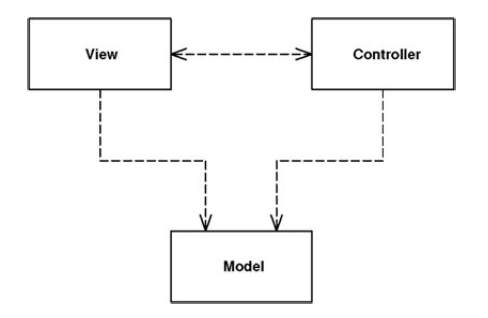
\includegraphics[width=0.80\textwidth]{img/MVC-Allgemein(Fowler).png}
\caption {MVC-Architektur}
\end{figure}
Wie auch in der Abbildung zu sehen, ist die Richtung der Abhängigkeiten für die MVC-Architektur entscheidend. Die Abbildung zeigt, dass sowohl View als auch Controller vom Model abhängig sind, jedoch keine Abhängigkeit des Models von View oder Controller besteht. Diese Unabhängigkeit des Models bedeutet, dass das Model auch bei Änderungen an View und Controller unverändert bleibt und damit Änderungen am View deutlich erleichtert.
(Patterns of Enterprise Application Architecture - Martin Fowler)
\subsection{ADF}
Dieses Kapitel soll einen Einblick in die Möglichkeiten des Frameworks ADF bieten und dessen Aufbau und Bedienbarkeit erläutern.

\subsubsection{Grundlegendes}

Eine Lösung zur Entwicklung von modernen Anwendungen als komponentenbasierte Benutzerschnittstelle bietet ORACLE mit dem Application Development Framework (ADF). ADF ist ein Java EE (Java Enterprise Edition) Framework, das Anwendungsentwicklung mit Java, Java EE und SOA vereinfachen soll um ein breites Publikum von Geschäftsbereich und Technologie Experten anzusprechen, die zusammen arbeiten müssen, um langlebige Enterprise Softwarelösungen entwickeln zu können.(Oracle Fusion Developer Guide Introduction Seite xxiii)
\subsubsection{Architektur}
\begin{figure}
\centering
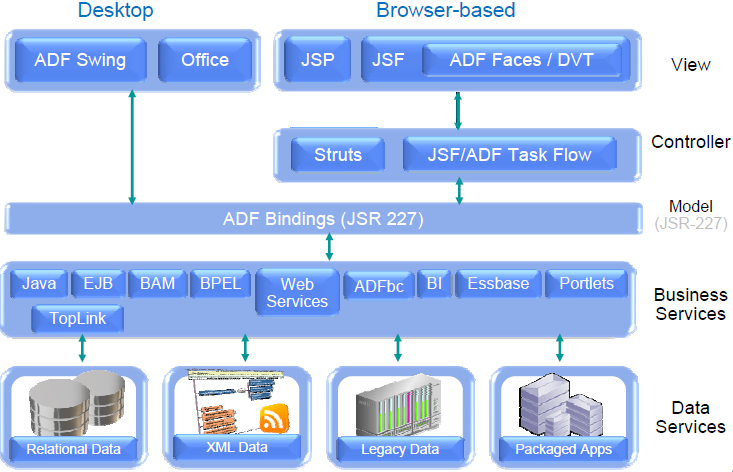
\includegraphics[width=0.80\textwidth]{img/MVC-ADF.png}
\caption {MVC-Architektur von ADF}
\end{figure}
\subsection{Grails}
Dieses Kapitel soll einen Einblick in das Framework Grails ermöglichen.
